\section{Auswertung}
\label{sec:Auswertung}

    \subsection{Kritische Parameter von \(SF_6\)}
    \label{subsec:KritischeParameter}

    Es wurde wie in \ref{sec:Experiment} beschrieben für 7 verschiedene Temperaturen die p-V-Abhängigkeit gemessen und in Abb. \ref{fig:pVDiagramm} graphisch dargestellt.
    \begin{figure}[H]
        \centering
        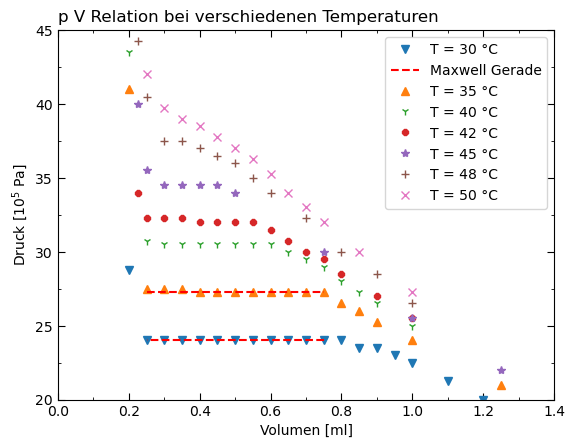
\includegraphics[width=0.4\textwidth]{../Images/pV_all.png}
        \caption{Auftragung der Isothermen von \(SF_6\) mit eingezeichneten Maxwell Geraden, bis auf bei \(T = 50 ^\circ C\), da hier der kritische Punkt überschritten wurde}
        \label{fig:pVDiagramm}
    \end{figure}

    Die Maxwell Gerade zeigt den Bereich, in dem das Gas sowohl flüssig als auch gasförmig vorliegt. Je weiter die Temperatur von der 
    kritischen Temperatur \(T_K\) entfernt ist, desto ausgeprägter ist dieser Bereich (vgl. \ref{fig:pVDiagramm}). \\
    Bei der Isothermen der kritische Temperatur \(T_K\) ist erkennbar, dass die anstatt eines Plateaus ein Sattelpunkt Höhe ders kritischen Volumens \(V_K\) und des kritischen Drucks \(p_K\) vorliegt. 

    \begin{equation}
        \frac{dp}{dV} = 0 |_{V=V_K} \quad \text{und} \quad \frac{d^2p}{dV^2} = 0 |_{V=V_K}
    \label{eq:Ableitungen}
    \end{equation}

    Die Start- und Endvolumina der Maxwell-Geraden wurden experimentell beobachtet. Aus diesen Volumina und den zugehörigen
    Drücken die kritischen Parameter \(p_K\) und \(V_K\) zu bestimmen, werden diese linear gefittet und aus dem Schnittpunkt der Geraden
    die Parameter bestimmt. Obwohl der reale Verlauf der Isothermen im Koexistenzbereich nicht linear ist,
    lassen sich die kritischen Parameter durch die Nutzung der Start- und Endwerte der Maxwell-Gerade gut annähern.
    Das funktioniert, da in diesen Bereichen eine lineare Näherung hinreichend genau ist.
    Daraus ergeben sich für die kritischen Parameter \(T_K\), \(p_K\) und \(V_K\) folgende Werte:

    \begin{equation}
        p_K = (38,5 \pm 4,0) \, \text{bar} \\
        V_K = (0,32 \pm 0,14) \, \text{cm}^3
    \end{equation}

    \textcolor{red}{BILD EINFÜGEN VON SCHNITTPUNKT}
    
    Der kritische Druck stimmt innerhalb des Fehlers mit dem Literaturwert von \(p_{K,lit} = 37,53 \, \text{bar}\) überein \cite{SF6LITERATUR} überein.
    Um das kritische Volumen mit dem Literaturwert vergleichen zu können, muss dieses noch in die Einheiten \(ml/mol\) umgerechnet werden.
    Die Stoffmenge ist ebenfalls experimentell bestimmt worden.
    \begin{equation}
        V_{K,mol} = (\textcolor{red}{HIER UMRECHNEN}) \frac{m^3}{mol}
    \end{equation}
    \subsection{Ermittlung der Dampfdruckkurve}

    \subsection{Ermittlung der Konstanten \(a\) und \(b\) der Van-der-Waals-Gleichung und des kritischen Koeffizienten \(K_K\)}
     
    Mit den Gleichungen \ref{eq:VanDerWaals} und \ref{eq:Ableitungen} lassen sich die Konstanten \(a\) und \(b\) bestimmen.

    \begin{equation}
        a = \frac{27 R^2 T_K^2}{64 p_K} = (78,1 \pm 9,7) \cdot 10^{3} \, J^2 \frac{ml}{mol^2}
    \label{eq:KonstanteA}
    \end{equation}

    \begin{equation}
        b = \frac{R T_K}{8 p_K} = (8,67 \pm 0,95) \, \frac{ml}{mol}
    \label{eq:KonstanteB}
    \end{equation}
    Der kritische Koeffizient \(K_K\) ergibt sich aus dem Verhältnis der kritischen Parameter:
    \begin{equation}
        K_K = \frac{R T_K} = (217 \pm 91)
    \label{eq:KritischerKoeffizient}
    \end{equation}
    
    
    \textcolor{red}{VGL MIT LITERATURWERTE}
